% Data flow diagram
% Author: David Fokkema
\documentclass{article}
\usepackage{tikz}
\usetikzlibrary{shapes,arrows}
\usepackage{pdflscape}
\usepackage[papersize={6.5cm, 9.6cm}, text={6.5cm, 9.2cm}]{geometry}
\usetikzlibrary{decorations.text}
\usepackage{xcolor}
% \selectcolormodel{gray}

\begin{document}
\thispagestyle{empty}
%\begin{landscape}
\begin{center}
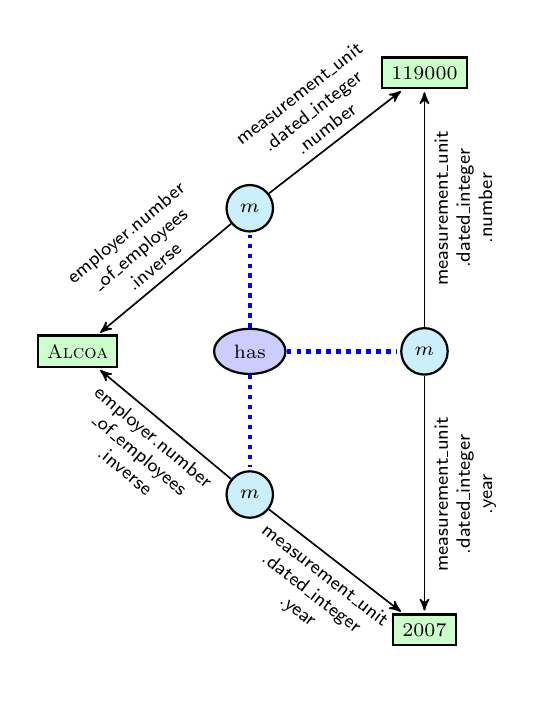
\begin{tikzpicture}[
  font=\sffamily,
  every matrix/.style={ampersand replacement=\&,column sep=1.2cm,row sep=1.2cm,font=\scriptsize},
  entity/.style={draw,thick,rectangle,fill=green!20},
  word/.style={draw,thick,ellipse,fill=blue!20},
  mediator/.style={draw,thick,circle},
  mediatorR/.style={draw,thick,circle,fill=cyan!20},
  mediatorV/.style={draw,thick,circle,fill=violet!20},
  mediatorY/.style={draw,thick,circle,fill=yellow!20},
  entityType/.style={draw,thick,rounded corners,fill=yellow!20,inner sep=.3cm},
  mathType/.style={draw,thick,diamond,fill=red!20},
  mediatorToEntity/.style={->,>=stealth',shorten >=1pt,semithick,black,sloped,above,font=\sffamily\scriptsize},
  typeToEntity/.style={->,>=stealth',shorten >=1pt,semithick,black,sloped,above,font=\sffamily\scriptsize},
  wordToEntity/.style={-,>=stealth',shorten >=1pt,ultra thick,dotted,blue,sloped,above,font=\sffamily\scriptsize},
  entityToMath/.style={->,>=stealth',shorten >=1pt,ultra thick,dashed,violet,sloped,above,font=\sffamily\scriptsize},
  every node/.style={align=center}]

  % Alcoa has 120,000 employees in 2007.
  
  % Position the nodes using a matrix layout
  \matrix{ 
    \&  \& \node[entity] (e120000) {119000}; \\
     \& \node[mediatorR] (m1) {$m$}; \&  \\
    \node[entity] (eAlcoa) {\textsc{Alcoa}}; \& \node[word] (wHas)
{has}; \& \node[mediatorR]
(m2)
{$m$}; \\
     \& \node[mediatorR] (m3) {$m$}; \&  \\
     \&  \& \node[entity] (e2007) {2007}; \\
  };
 
  % words to entities
  % \draw [wordToEntity] (wAlcoa) edge node {}  (eAlcoa);
  % \draw [wordToEntity] (w120000) edge node {}  (e120000);
  % \draw [wordToEntity] (w2007) edge node {}  (e2007);
  
  % event word to mediators
   \draw [wordToEntity] (wHas) edge node {}  (m1);
   \draw [wordToEntity] (wHas) edge node {}  (m2);
   \draw [wordToEntity] (wHas) edge node {}  (m3);
  
  % mediator to entities
  \draw [mediatorToEntity] (m1) edge node {employer.number\\\_of\_employees\\.inverse} 
(eAlcoa);
  \draw [mediatorToEntity] (m1) edge node {measurement\_unit\\.dated\_integer\\.number} 
(e120000);
  
  \draw [mediatorToEntity] (m2) edge node[below,rotate=180] {measurement\_unit\\.dated\_integer\\.year}  (e2007);
  \draw [mediatorToEntity] (m2) edge node[below] {measurement\_unit\\.dated\_integer\\.number}  (e120000);
  
  \draw [mediatorToEntity] (m3) edge node[below] {employer.number\\\_of\_employees\\.inverse}  (eAlcoa);
  \draw [mediatorToEntity] (m3) edge node[below] {measurement\_unit\\.dated\_integer\\.year}  (e2007);
  
  
  
\end{tikzpicture} 
\scriptsize $\mbox{employer.number\_of\_employees.inverse}(m, \textsc{Alcoa}) \wedge
 \mbox{measurement\_unit.dated\_integer.number}(m, 119000) $
 $\wedge\; \mbox{measurement\_unit.dated\_integer.year}(m, 2007)$
\end{center}


\end{document}
